%-------------------------------------------------------------------------------
%                            BAB III
%               		METODOLOGI PENELITIAN
%-------------------------------------------------------------------------------
% \fancyhf{} 
% \fancyfoot[C]{\thepage}
\captionsetup[figure]{labelfont={normalfont}, textfont={normalfont}}

\chapter{METODOLOGI PENELITIAN}
%\usepackage{table,xcdraw}[xcolor]
%\thispagestyle{plain} % Halaman pertama bab menggunakan gaya plain

\section{Waktu dan Lokasi Penelitian}
Penelitian ini akan bertempat di Ruang Lab Sistem Informasi dan \textit{Database}. Waktu yang dibutuhkan agar penelitian ini dapat diimplementasikan adalah 4 bulan terhitung dari bulan Februari 2024 hingga Mei 2024.

\section{Jadwal Pelaksanaan}

\par Untuk lebih memahami alur waktu dari penelitian ini, penulis telah menyusun sebuah jadwal yang rinci yang bisa dilihat pada Tabel \ref{tab:jadwal_pelaksanaan}.


% \begin{table}[H]
%     \centering
%     \caption{Jadwal Pelaksanaan Penelitian}
%     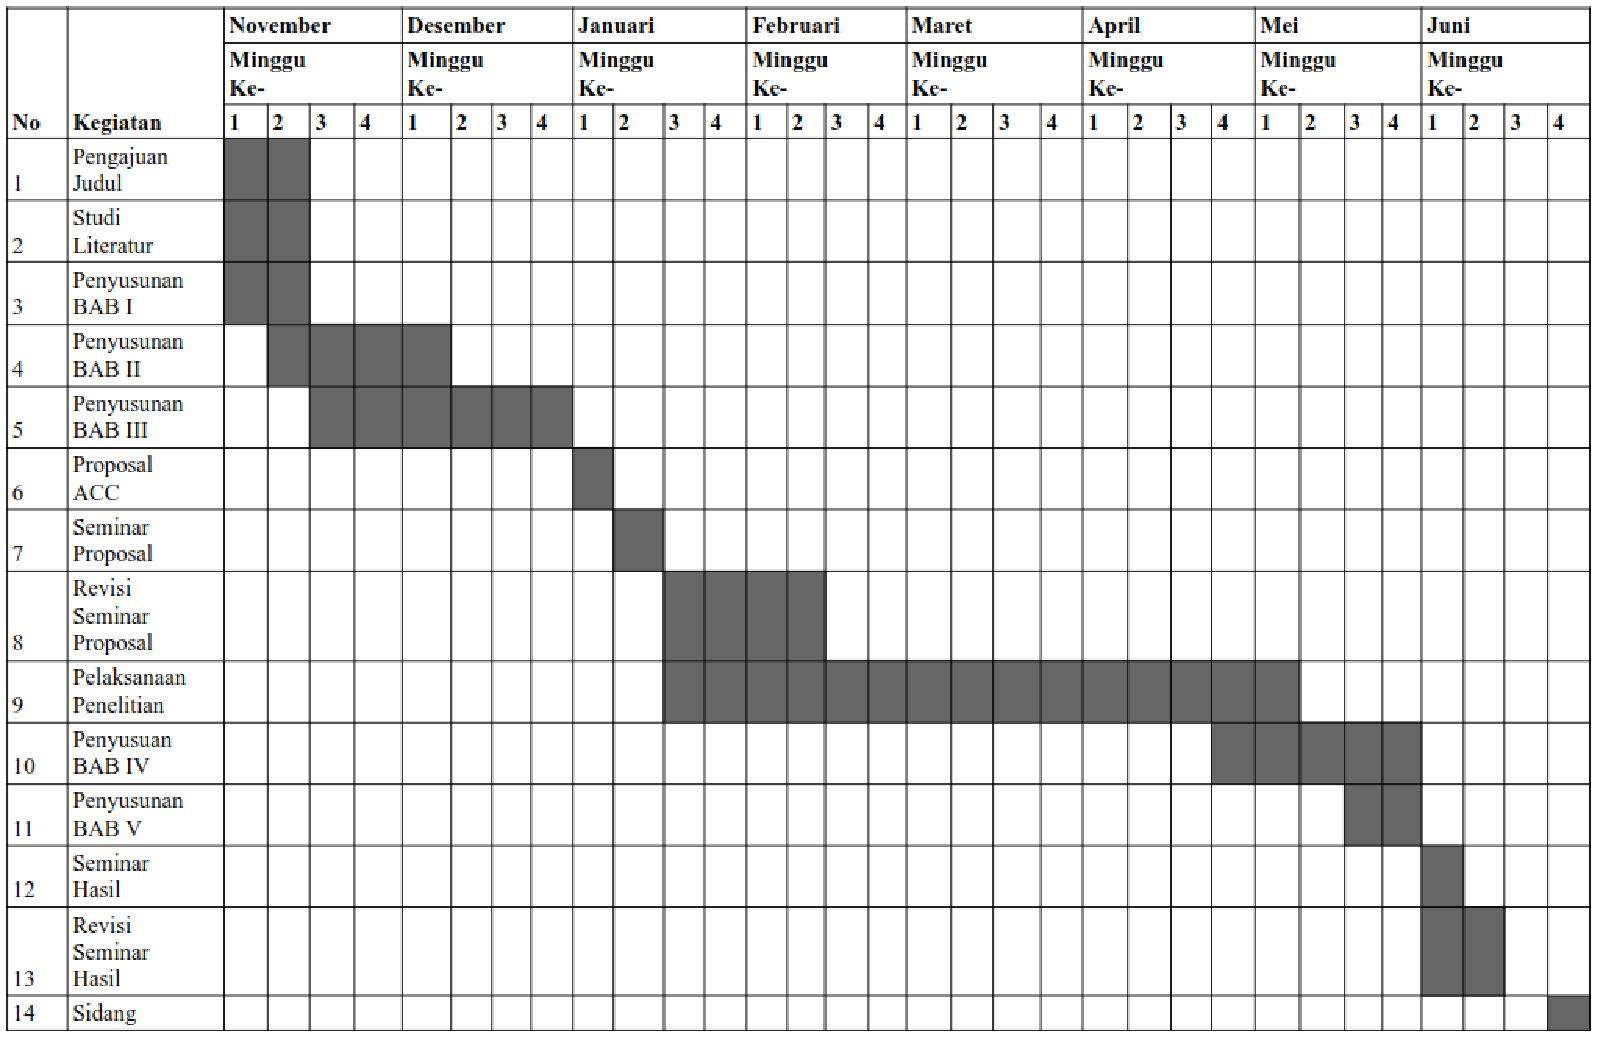
\includegraphics[width=\textwidth]{image/bab3/jadwal-pelaksanaan.pdf}\label{tab:jadwal_pelaksanaan}
% \end{table}


% Please add the following required packages to your document preamble:
% \usepackage{multirow}
% \usepackage{graphicx}
% \usepackage[table,xcdraw]{xcolor}
% Beamer presentation requires \usepackage{colortbl} instead of \usepackage[table,xcdraw]{xcolor}
\begin{table}[H]
  \centering
  \caption{Jadwal pelaksanaan penelitian}
  \label{tab:jadwal_pelaksanaan}
  \resizebox{\textwidth}{!}{%
  \begin{tabular}{|l|l|llllllllllllllllllllllll|}
  \hline
   &
     &
    \multicolumn{24}{c|}{\textbf{Bulan Ke -}} \\ \cline{3-26} 
   &
     &
    \multicolumn{4}{c|}{\textbf{Januari}} &
    \multicolumn{4}{c|}{\textbf{Februari}} &
    \multicolumn{4}{c|}{\textbf{Maret}} &
    \multicolumn{4}{c|}{\textbf{April}} &
    \multicolumn{4}{c|}{\textbf{Mei}} &
    \multicolumn{4}{c|}{\textbf{Juni}} \\ \cline{3-26} 
  \multirow{-3}{*}{\textbf{No}} &
    \multirow{-3}{*}{\textbf{Kegiatan}} &
    \multicolumn{1}{c|}{\textbf{1}} &
    \multicolumn{1}{c|}{\textbf{2}} &
    \multicolumn{1}{c|}{\textbf{3}} &
    \multicolumn{1}{c|}{\textbf{4}} &
    \multicolumn{1}{c|}{\textbf{1}} &
    \multicolumn{1}{c|}{\textbf{2}} &
    \multicolumn{1}{c|}{\textbf{3}} &
    \multicolumn{1}{c|}{\textbf{4}} &
    \multicolumn{1}{c|}{\textbf{1}} &
    \multicolumn{1}{c|}{\textbf{2}} &
    \multicolumn{1}{c|}{\textbf{3}} &
    \multicolumn{1}{c|}{\textbf{4}} &
    \multicolumn{1}{c|}{\textbf{1}} &
    \multicolumn{1}{c|}{\textbf{2}} &
    \multicolumn{1}{c|}{\textbf{3}} &
    \multicolumn{1}{c|}{\textbf{4}} &
    \multicolumn{1}{c|}{\textbf{1}} &
    \multicolumn{1}{c|}{\textbf{2}} &
    \multicolumn{1}{c|}{\textbf{3}} &
    \multicolumn{1}{c|}{\textbf{4}} &
    \multicolumn{1}{c|}{\textbf{1}} &
    \multicolumn{1}{c|}{\textbf{2}} &
    \multicolumn{1}{c|}{\textbf{3}} &
    \multicolumn{1}{c|}{\textbf{4}} \\ \hline
  1 &
    Studi literatur &
    \multicolumn{1}{l|}{\cellcolor[HTML]{333333}{\color[HTML]{333333} }} &
    \multicolumn{1}{l|}{\cellcolor[HTML]{333333}{\color[HTML]{333333} }} &
    \multicolumn{1}{l|}{\cellcolor[HTML]{333333}{\color[HTML]{333333} }} &
    \multicolumn{1}{l|}{\cellcolor[HTML]{333333}{\color[HTML]{333333} }} &
    \multicolumn{1}{l|}{} &
    \multicolumn{1}{l|}{} &
    \multicolumn{1}{l|}{} &
    \multicolumn{1}{l|}{} &
    \multicolumn{1}{l|}{} &
    \multicolumn{1}{l|}{} &
    \multicolumn{1}{l|}{} &
    \multicolumn{1}{l|}{} &
    \multicolumn{1}{l|}{} &
    \multicolumn{1}{l|}{} &
    \multicolumn{1}{l|}{} &
    \multicolumn{1}{l|}{} &
    \multicolumn{1}{l|}{} &
    \multicolumn{1}{l|}{} &
    \multicolumn{1}{l|}{} &
    \multicolumn{1}{l|}{} &
    \multicolumn{1}{l|}{} &
    \multicolumn{1}{l|}{} &
    \multicolumn{1}{l|}{} &
     \\ \hline
  2 &
    Pengumpulan data &
    \multicolumn{1}{l|}{} &
    \multicolumn{1}{l|}{} &
    \multicolumn{1}{l|}{\cellcolor[HTML]{333333}} &
    \multicolumn{1}{l|}{\cellcolor[HTML]{333333}} &
    \multicolumn{1}{l|}{\cellcolor[HTML]{333333}} &
    \multicolumn{1}{l|}{\cellcolor[HTML]{333333}} &
    \multicolumn{1}{l|}{} &
    \multicolumn{1}{l|}{} &
    \multicolumn{1}{l|}{} &
    \multicolumn{1}{l|}{} &
    \multicolumn{1}{l|}{} &
    \multicolumn{1}{l|}{} &
    \multicolumn{1}{l|}{} &
    \multicolumn{1}{l|}{} &
    \multicolumn{1}{l|}{} &
    \multicolumn{1}{l|}{} &
    \multicolumn{1}{l|}{} &
    \multicolumn{1}{l|}{} &
    \multicolumn{1}{l|}{} &
    \multicolumn{1}{l|}{} &
    \multicolumn{1}{l|}{} &
    \multicolumn{1}{l|}{} &
    \multicolumn{1}{l|}{} &
     \\ \hline
  3 &
    Pemrosesan data &
    \multicolumn{1}{l|}{} &
    \multicolumn{1}{l|}{} &
    \multicolumn{1}{l|}{} &
    \multicolumn{1}{l|}{} &
    \multicolumn{1}{l|}{\cellcolor[HTML]{333333}} &
    \multicolumn{1}{l|}{\cellcolor[HTML]{333333}} &
    \multicolumn{1}{l|}{\cellcolor[HTML]{333333}} &
    \multicolumn{1}{l|}{\cellcolor[HTML]{333333}} &
    \multicolumn{1}{l|}{\cellcolor[HTML]{333333}} &
    \multicolumn{1}{l|}{\cellcolor[HTML]{333333}} &
    \multicolumn{1}{l|}{} &
    \multicolumn{1}{l|}{} &
    \multicolumn{1}{l|}{} &
    \multicolumn{1}{l|}{} &
    \multicolumn{1}{l|}{} &
    \multicolumn{1}{l|}{} &
    \multicolumn{1}{l|}{} &
    \multicolumn{1}{l|}{} &
    \multicolumn{1}{l|}{} &
    \multicolumn{1}{l|}{} &
    \multicolumn{1}{l|}{} &
    \multicolumn{1}{l|}{} &
    \multicolumn{1}{l|}{} &
     \\ \hline
  4 &
    Membangun model &
    \multicolumn{1}{l|}{} &
    \multicolumn{1}{l|}{} &
    \multicolumn{1}{l|}{} &
    \multicolumn{1}{l|}{} &
    \multicolumn{1}{l|}{} &
    \multicolumn{1}{l|}{} &
    \multicolumn{1}{l|}{} &
    \multicolumn{1}{l|}{} &
    \multicolumn{1}{l|}{} &
    \multicolumn{1}{l|}{} &
    \multicolumn{1}{l|}{\cellcolor[HTML]{333333}} &
    \multicolumn{1}{l|}{\cellcolor[HTML]{333333}} &
    \multicolumn{1}{l|}{} &
    \multicolumn{1}{l|}{} &
    \multicolumn{1}{l|}{} &
    \multicolumn{1}{l|}{} &
    \multicolumn{1}{l|}{} &
    \multicolumn{1}{l|}{} &
    \multicolumn{1}{l|}{} &
    \multicolumn{1}{l|}{} &
    \multicolumn{1}{l|}{} &
    \multicolumn{1}{l|}{} &
    \multicolumn{1}{l|}{} &
     \\ \hline
  5 &
    Melatih model &
    \multicolumn{1}{l|}{} &
    \multicolumn{1}{l|}{} &
    \multicolumn{1}{l|}{} &
    \multicolumn{1}{l|}{} &
    \multicolumn{1}{l|}{} &
    \multicolumn{1}{l|}{} &
    \multicolumn{1}{l|}{} &
    \multicolumn{1}{l|}{} &
    \multicolumn{1}{l|}{} &
    \multicolumn{1}{l|}{} &
    \multicolumn{1}{l|}{} &
    \multicolumn{1}{l|}{\cellcolor[HTML]{333333}} &
    \multicolumn{1}{l|}{\cellcolor[HTML]{333333}} &
    \multicolumn{1}{l|}{\cellcolor[HTML]{333333}} &
    \multicolumn{1}{l|}{\cellcolor[HTML]{333333}} &
    \multicolumn{1}{l|}{\cellcolor[HTML]{333333}} &
    \multicolumn{1}{l|}{\cellcolor[HTML]{333333}} &
    \multicolumn{1}{l|}{\cellcolor[HTML]{333333}} &
    \multicolumn{1}{l|}{} &
    \multicolumn{1}{l|}{} &
    \multicolumn{1}{l|}{} &
    \multicolumn{1}{l|}{} &
    \multicolumn{1}{l|}{} &
     \\ \hline
  6 &
    Analisis hasil &
    \multicolumn{1}{l|}{} &
    \multicolumn{1}{l|}{} &
    \multicolumn{1}{l|}{} &
    \multicolumn{1}{l|}{} &
    \multicolumn{1}{l|}{} &
    \multicolumn{1}{l|}{} &
    \multicolumn{1}{l|}{} &
    \multicolumn{1}{l|}{} &
    \multicolumn{1}{l|}{} &
    \multicolumn{1}{l|}{} &
    \multicolumn{1}{l|}{} &
    \multicolumn{1}{l|}{} &
    \multicolumn{1}{l|}{} &
    \multicolumn{1}{l|}{} &
    \multicolumn{1}{l|}{} &
    \multicolumn{1}{l|}{} &
    \multicolumn{1}{l|}{} &
    \multicolumn{1}{l|}{} &
    \multicolumn{1}{l|}{\cellcolor[HTML]{333333}} &
    \multicolumn{1}{l|}{} &
    \multicolumn{1}{l|}{} &
    \multicolumn{1}{l|}{} &
    \multicolumn{1}{l|}{} &
     \\ \hline
  7 &
    Penyusunan laporan akhir &
    \multicolumn{1}{l|}{} &
    \multicolumn{1}{l|}{} &
    \multicolumn{1}{l|}{} &
    \multicolumn{1}{l|}{} &
    \multicolumn{1}{l|}{} &
    \multicolumn{1}{l|}{} &
    \multicolumn{1}{l|}{} &
    \multicolumn{1}{l|}{} &
    \multicolumn{1}{l|}{} &
    \multicolumn{1}{l|}{} &
    \multicolumn{1}{l|}{} &
    \multicolumn{1}{l|}{} &
    \multicolumn{1}{l|}{} &
    \multicolumn{1}{l|}{} &
    \multicolumn{1}{l|}{} &
    \multicolumn{1}{l|}{} &
    \multicolumn{1}{l|}{} &
    \multicolumn{1}{l|}{} &
    \multicolumn{1}{l|}{} &
    \multicolumn{1}{l|}{\cellcolor[HTML]{333333}} &
    \multicolumn{1}{l|}{\cellcolor[HTML]{333333}} &
    \multicolumn{1}{l|}{\cellcolor[HTML]{333333}} &
    \multicolumn{1}{l|}{} &
     \\ \hline
  \end{tabular}%
  }
  \end{table}


% Please add the following required packages to your document preamble:
% \usepackage{multirow}
% \usepackage{graphicx}
% \usepackage[table,xcdraw]{xcolor}
% Beamer presentation requires \usepackage{colortbl} instead of \usepackage[table,xcdraw]{xcolor}
% \begin{table}[H]
%     \centering
%     \caption{Jadwal pelaksanaan penelitian}
%     \label{tab: jadwal-pelaksanaan}
%     \resizebox{\textwidth}{!}{%
%     \begin{tabular}{|l|l|llll|llll|llll|llll|llll|llll|llll|llll|}
%     \hline
%      &
%        &
%       \multicolumn{4}{l|}{\textbf{November}} &
%       \multicolumn{4}{l|}{\textbf{Desember}} &
%       \multicolumn{4}{l|}{\textbf{Januari}} &
%       \multicolumn{4}{l|}{\textbf{Februari}} &
%       \multicolumn{4}{l|}{\textbf{Maret}} &
%       \multicolumn{4}{l|}{\textbf{April}} &
%       \multicolumn{4}{l|}{\textbf{Mei}} &
%       \multicolumn{4}{l|}{\textbf{Juni}} \\ \cline{3-34} 
%      &
%        &
%       \multicolumn{4}{l|}{\textbf{\begin{tabular}[c]{@{}l@{}}Minggu\\ Ke-\end{tabular}}} &
%       \multicolumn{4}{l|}{\textbf{\begin{tabular}[c]{@{}l@{}}Minggu\\ Ke-\end{tabular}}} &
%       \multicolumn{4}{l|}{\textbf{\begin{tabular}[c]{@{}l@{}}Minggu\\ Ke-\end{tabular}}} &
%       \multicolumn{4}{l|}{\textbf{\begin{tabular}[c]{@{}l@{}}Minggu\\ Ke-\end{tabular}}} &
%       \multicolumn{4}{l|}{\textbf{\begin{tabular}[c]{@{}l@{}}Minggu\\ Ke-\end{tabular}}} &
%       \multicolumn{4}{l|}{\textbf{\begin{tabular}[c]{@{}l@{}}Minggu\\ Ke-\end{tabular}}} &
%       \multicolumn{4}{l|}{\textbf{\begin{tabular}[c]{@{}l@{}}Minggu\\ Ke-\end{tabular}}} &
%       \multicolumn{4}{l|}{\textbf{\begin{tabular}[c]{@{}l@{}}Minggu\\ Ke-\end{tabular}}} \\ \cline{3-34} 
%     \multirow{-3}{*}{\textbf{No}} &
%       \multirow{-3}{*}{\textbf{Kegiatan}} &
%       \multicolumn{1}{l|}{\textbf{1}} &
%       \multicolumn{1}{l|}{\textbf{2}} &
%       \multicolumn{1}{l|}{\textbf{3}} &
%       \textbf{4} &
%       \multicolumn{1}{l|}{\textbf{1}} &
%       \multicolumn{1}{l|}{\textbf{2}} &
%       \multicolumn{1}{l|}{\textbf{3}} &
%       \textbf{4} &
%       \multicolumn{1}{l|}{\textbf{1}} &
%       \multicolumn{1}{l|}{\textbf{2}} &
%       \multicolumn{1}{l|}{\textbf{3}} &
%       \textbf{4} &
%       \multicolumn{1}{l|}{\textbf{1}} &
%       \multicolumn{1}{l|}{\textbf{2}} &
%       \multicolumn{1}{l|}{\textbf{3}} &
%       \textbf{4} &
%       \multicolumn{1}{l|}{\textbf{1}} &
%       \multicolumn{1}{l|}{\textbf{2}} &
%       \multicolumn{1}{l|}{\textbf{3}} &
%       \textbf{4} &
%       \multicolumn{1}{l|}{\textbf{1}} &
%       \multicolumn{1}{l|}{\textbf{2}} &
%       \multicolumn{1}{l|}{\textbf{3}} &
%       \textbf{4} &
%       \multicolumn{1}{l|}{\textbf{1}} &
%       \multicolumn{1}{l|}{\textbf{2}} &
%       \multicolumn{1}{l|}{\textbf{3}} &
%       \textbf{4} &
%       \multicolumn{1}{l|}{\textbf{1}} &
%       \multicolumn{1}{l|}{\textbf{2}} &
%       \multicolumn{1}{l|}{\textbf{3}} &
%       \textbf{4} \\ \hline
%     1 &
%       \begin{tabular}[c]{@{}l@{}}Pengajuan \\ Judul\end{tabular} &
%       \multicolumn{1}{l|}{\cellcolor[HTML]{666666}} &
%       \multicolumn{1}{l|}{\cellcolor[HTML]{666666}} &
%       \multicolumn{1}{l|}{} &
%        &
%       \multicolumn{1}{l|}{} &
%       \multicolumn{1}{l|}{} &
%       \multicolumn{1}{l|}{} &
%        &
%       \multicolumn{1}{l|}{} &
%       \multicolumn{1}{l|}{} &
%       \multicolumn{1}{l|}{} &
%        &
%       \multicolumn{1}{l|}{} &
%       \multicolumn{1}{l|}{} &
%       \multicolumn{1}{l|}{} &
%        &
%       \multicolumn{1}{l|}{} &
%       \multicolumn{1}{l|}{} &
%       \multicolumn{1}{l|}{} &
%        &
%       \multicolumn{1}{l|}{} &
%       \multicolumn{1}{l|}{} &
%       \multicolumn{1}{l|}{} &
%        &
%       \multicolumn{1}{l|}{} &
%       \multicolumn{1}{l|}{} &
%       \multicolumn{1}{l|}{} &
%        &
%       \multicolumn{1}{l|}{} &
%       \multicolumn{1}{l|}{} &
%       \multicolumn{1}{l|}{} &
%        \\ \hline
%     2 &
%       \begin{tabular}[c]{@{}l@{}}Studi \\ Literatur\end{tabular} &
%       \multicolumn{1}{l|}{\cellcolor[HTML]{666666}} &
%       \multicolumn{1}{l|}{\cellcolor[HTML]{666666}} &
%       \multicolumn{1}{l|}{} &
%        &
%       \multicolumn{1}{l|}{} &
%       \multicolumn{1}{l|}{} &
%       \multicolumn{1}{l|}{} &
%        &
%       \multicolumn{1}{l|}{} &
%       \multicolumn{1}{l|}{} &
%       \multicolumn{1}{l|}{} &
%        &
%       \multicolumn{1}{l|}{} &
%       \multicolumn{1}{l|}{} &
%       \multicolumn{1}{l|}{} &
%        &
%       \multicolumn{1}{l|}{} &
%       \multicolumn{1}{l|}{} &
%       \multicolumn{1}{l|}{} &
%        &
%       \multicolumn{1}{l|}{} &
%       \multicolumn{1}{l|}{} &
%       \multicolumn{1}{l|}{} &
%        &
%       \multicolumn{1}{l|}{} &
%       \multicolumn{1}{l|}{} &
%       \multicolumn{1}{l|}{} &
%        &
%       \multicolumn{1}{l|}{} &
%       \multicolumn{1}{l|}{} &
%       \multicolumn{1}{l|}{} &
%        \\ \hline
%     3 &
%       \begin{tabular}[c]{@{}l@{}}Penyusunan \\ BAB I\end{tabular} &
%       \multicolumn{1}{l|}{\cellcolor[HTML]{666666}} &
%       \multicolumn{1}{l|}{\cellcolor[HTML]{666666}} &
%       \multicolumn{1}{l|}{} &
%        &
%       \multicolumn{1}{l|}{} &
%       \multicolumn{1}{l|}{} &
%       \multicolumn{1}{l|}{} &
%        &
%       \multicolumn{1}{l|}{} &
%       \multicolumn{1}{l|}{} &
%       \multicolumn{1}{l|}{} &
%        &
%       \multicolumn{1}{l|}{} &
%       \multicolumn{1}{l|}{} &
%       \multicolumn{1}{l|}{} &
%        &
%       \multicolumn{1}{l|}{} &
%       \multicolumn{1}{l|}{} &
%       \multicolumn{1}{l|}{} &
%        &
%       \multicolumn{1}{l|}{} &
%       \multicolumn{1}{l|}{} &
%       \multicolumn{1}{l|}{} &
%        &
%       \multicolumn{1}{l|}{} &
%       \multicolumn{1}{l|}{} &
%       \multicolumn{1}{l|}{} &
%        &
%       \multicolumn{1}{l|}{} &
%       \multicolumn{1}{l|}{} &
%       \multicolumn{1}{l|}{} &
%        \\ \hline
%     4 &
%       \begin{tabular}[c]{@{}l@{}}Penyusunan \\ BAB II\end{tabular} &
%       \multicolumn{1}{l|}{} &
%       \multicolumn{1}{l|}{\cellcolor[HTML]{666666}} &
%       \multicolumn{1}{l|}{\cellcolor[HTML]{666666}} &
%       \cellcolor[HTML]{666666} &
%       \multicolumn{1}{l|}{\cellcolor[HTML]{666666}} &
%       \multicolumn{1}{l|}{} &
%       \multicolumn{1}{l|}{} &
%        &
%       \multicolumn{1}{l|}{} &
%       \multicolumn{1}{l|}{} &
%       \multicolumn{1}{l|}{} &
%        &
%       \multicolumn{1}{l|}{} &
%       \multicolumn{1}{l|}{} &
%       \multicolumn{1}{l|}{} &
%        &
%       \multicolumn{1}{l|}{} &
%       \multicolumn{1}{l|}{} &
%       \multicolumn{1}{l|}{} &
%        &
%       \multicolumn{1}{l|}{} &
%       \multicolumn{1}{l|}{} &
%       \multicolumn{1}{l|}{} &
%        &
%       \multicolumn{1}{l|}{} &
%       \multicolumn{1}{l|}{} &
%       \multicolumn{1}{l|}{} &
%        &
%       \multicolumn{1}{l|}{} &
%       \multicolumn{1}{l|}{} &
%       \multicolumn{1}{l|}{} &
%        \\ \hline
%     5 &
%       \begin{tabular}[c]{@{}l@{}}Penyusunan \\ BAB III\end{tabular} &
%       \multicolumn{1}{l|}{} &
%       \multicolumn{1}{l|}{} &
%       \multicolumn{1}{l|}{\cellcolor[HTML]{666666}} &
%       \cellcolor[HTML]{666666} &
%       \multicolumn{1}{l|}{\cellcolor[HTML]{666666}} &
%       \multicolumn{1}{l|}{\cellcolor[HTML]{666666}} &
%       \multicolumn{1}{l|}{\cellcolor[HTML]{666666}} &
%       \cellcolor[HTML]{666666} &
%       \multicolumn{1}{l|}{} &
%       \multicolumn{1}{l|}{} &
%       \multicolumn{1}{l|}{} &
%        &
%       \multicolumn{1}{l|}{} &
%       \multicolumn{1}{l|}{} &
%       \multicolumn{1}{l|}{} &
%        &
%       \multicolumn{1}{l|}{} &
%       \multicolumn{1}{l|}{} &
%       \multicolumn{1}{l|}{} &
%        &
%       \multicolumn{1}{l|}{} &
%       \multicolumn{1}{l|}{} &
%       \multicolumn{1}{l|}{} &
%        &
%       \multicolumn{1}{l|}{} &
%       \multicolumn{1}{l|}{} &
%       \multicolumn{1}{l|}{} &
%        &
%       \multicolumn{1}{l|}{} &
%       \multicolumn{1}{l|}{} &
%       \multicolumn{1}{l|}{} &
%        \\ \hline
%     6 &
%       \begin{tabular}[c]{@{}l@{}}Proposal \\ ACC\end{tabular} &
%       \multicolumn{1}{l|}{} &
%       \multicolumn{1}{l|}{} &
%       \multicolumn{1}{l|}{} &
%        &
%       \multicolumn{1}{l|}{} &
%       \multicolumn{1}{l|}{} &
%       \multicolumn{1}{l|}{} &
%        &
%       \multicolumn{1}{l|}{\cellcolor[HTML]{666666}} &
%       \multicolumn{1}{l|}{} &
%       \multicolumn{1}{l|}{} &
%        &
%       \multicolumn{1}{l|}{} &
%       \multicolumn{1}{l|}{} &
%       \multicolumn{1}{l|}{} &
%        &
%       \multicolumn{1}{l|}{} &
%       \multicolumn{1}{l|}{} &
%       \multicolumn{1}{l|}{} &
%        &
%       \multicolumn{1}{l|}{} &
%       \multicolumn{1}{l|}{} &
%       \multicolumn{1}{l|}{} &
%        &
%       \multicolumn{1}{l|}{} &
%       \multicolumn{1}{l|}{} &
%       \multicolumn{1}{l|}{} &
%        &
%       \multicolumn{1}{l|}{} &
%       \multicolumn{1}{l|}{} &
%       \multicolumn{1}{l|}{} &
%        \\ \hline
%     7 &
%       \begin{tabular}[c]{@{}l@{}}Seminar \\ Proposal\end{tabular} &
%       \multicolumn{1}{l|}{} &
%       \multicolumn{1}{l|}{} &
%       \multicolumn{1}{l|}{} &
%        &
%       \multicolumn{1}{l|}{} &
%       \multicolumn{1}{l|}{} &
%       \multicolumn{1}{l|}{} &
%        &
%       \multicolumn{1}{l|}{} &
%       \multicolumn{1}{l|}{\cellcolor[HTML]{666666}} &
%       \multicolumn{1}{l|}{} &
%        &
%       \multicolumn{1}{l|}{} &
%       \multicolumn{1}{l|}{} &
%       \multicolumn{1}{l|}{} &
%        &
%       \multicolumn{1}{l|}{} &
%       \multicolumn{1}{l|}{} &
%       \multicolumn{1}{l|}{} &
%        &
%       \multicolumn{1}{l|}{} &
%       \multicolumn{1}{l|}{} &
%       \multicolumn{1}{l|}{} &
%        &
%       \multicolumn{1}{l|}{} &
%       \multicolumn{1}{l|}{} &
%       \multicolumn{1}{l|}{} &
%        &
%       \multicolumn{1}{l|}{} &
%       \multicolumn{1}{l|}{} &
%       \multicolumn{1}{l|}{} &
%        \\ \hline
%     8 &
%       \begin{tabular}[c]{@{}l@{}}Revisi \\ Seminar \\ Proposal\end{tabular} &
%       \multicolumn{1}{l|}{} &
%       \multicolumn{1}{l|}{} &
%       \multicolumn{1}{l|}{} &
%        &
%       \multicolumn{1}{l|}{} &
%       \multicolumn{1}{l|}{} &
%       \multicolumn{1}{l|}{} &
%        &
%       \multicolumn{1}{l|}{} &
%       \multicolumn{1}{l|}{} &
%       \multicolumn{1}{l|}{\cellcolor[HTML]{666666}} &
%       \cellcolor[HTML]{666666} &
%       \multicolumn{1}{l|}{\cellcolor[HTML]{666666}} &
%       \multicolumn{1}{l|}{\cellcolor[HTML]{666666}} &
%       \multicolumn{1}{l|}{} &
%        &
%       \multicolumn{1}{l|}{} &
%       \multicolumn{1}{l|}{} &
%       \multicolumn{1}{l|}{} &
%        &
%       \multicolumn{1}{l|}{} &
%       \multicolumn{1}{l|}{} &
%       \multicolumn{1}{l|}{} &
%        &
%       \multicolumn{1}{l|}{} &
%       \multicolumn{1}{l|}{} &
%       \multicolumn{1}{l|}{} &
%        &
%       \multicolumn{1}{l|}{} &
%       \multicolumn{1}{l|}{} &
%       \multicolumn{1}{l|}{} &
%        \\ \hline
%     9 &
%       \begin{tabular}[c]{@{}l@{}}Pelaksanaan \\ Penelitian\end{tabular} &
%       \multicolumn{1}{l|}{} &
%       \multicolumn{1}{l|}{} &
%       \multicolumn{1}{l|}{} &
%        &
%       \multicolumn{1}{l|}{} &
%       \multicolumn{1}{l|}{} &
%       \multicolumn{1}{l|}{} &
%        &
%       \multicolumn{1}{l|}{} &
%       \multicolumn{1}{l|}{} &
%       \multicolumn{1}{l|}{\cellcolor[HTML]{666666}} &
%       \cellcolor[HTML]{666666} &
%       \multicolumn{1}{l|}{\cellcolor[HTML]{666666}} &
%       \multicolumn{1}{l|}{\cellcolor[HTML]{666666}} &
%       \multicolumn{1}{l|}{\cellcolor[HTML]{666666}} &
%       \cellcolor[HTML]{666666} &
%       \multicolumn{1}{l|}{\cellcolor[HTML]{666666}} &
%       \multicolumn{1}{l|}{\cellcolor[HTML]{666666}} &
%       \multicolumn{1}{l|}{\cellcolor[HTML]{666666}} &
%       \cellcolor[HTML]{666666} &
%       \multicolumn{1}{l|}{\cellcolor[HTML]{666666}} &
%       \multicolumn{1}{l|}{\cellcolor[HTML]{666666}} &
%       \multicolumn{1}{l|}{\cellcolor[HTML]{666666}} &
%       \cellcolor[HTML]{666666} &
%       \multicolumn{1}{l|}{\cellcolor[HTML]{666666}} &
%       \multicolumn{1}{l|}{} &
%       \multicolumn{1}{l|}{} &
%        &
%       \multicolumn{1}{l|}{} &
%       \multicolumn{1}{l|}{} &
%       \multicolumn{1}{l|}{} &
%        \\ \hline
%     10 &
%       \begin{tabular}[c]{@{}l@{}}Penyusuan \\ BAB IV\end{tabular} &
%       \multicolumn{1}{l|}{} &
%       \multicolumn{1}{l|}{} &
%       \multicolumn{1}{l|}{} &
%        &
%       \multicolumn{1}{l|}{} &
%       \multicolumn{1}{l|}{} &
%       \multicolumn{1}{l|}{} &
%        &
%       \multicolumn{1}{l|}{} &
%       \multicolumn{1}{l|}{} &
%       \multicolumn{1}{l|}{} &
%        &
%       \multicolumn{1}{l|}{} &
%       \multicolumn{1}{l|}{} &
%       \multicolumn{1}{l|}{} &
%        &
%       \multicolumn{1}{l|}{} &
%       \multicolumn{1}{l|}{} &
%       \multicolumn{1}{l|}{} &
%        &
%       \multicolumn{1}{l|}{} &
%       \multicolumn{1}{l|}{} &
%       \multicolumn{1}{l|}{} &
%       \cellcolor[HTML]{666666} &
%       \multicolumn{1}{l|}{\cellcolor[HTML]{666666}} &
%       \multicolumn{1}{l|}{\cellcolor[HTML]{666666}} &
%       \multicolumn{1}{l|}{\cellcolor[HTML]{666666}} &
%       \cellcolor[HTML]{666666} &
%       \multicolumn{1}{l|}{} &
%       \multicolumn{1}{l|}{} &
%       \multicolumn{1}{l|}{} &
%        \\ \hline
%     11 &
%       \begin{tabular}[c]{@{}l@{}}Penyusunan \\ BAB V\end{tabular} &
%       \multicolumn{1}{l|}{} &
%       \multicolumn{1}{l|}{} &
%       \multicolumn{1}{l|}{} &
%        &
%       \multicolumn{1}{l|}{} &
%       \multicolumn{1}{l|}{} &
%       \multicolumn{1}{l|}{} &
%        &
%       \multicolumn{1}{l|}{} &
%       \multicolumn{1}{l|}{} &
%       \multicolumn{1}{l|}{} &
%        &
%       \multicolumn{1}{l|}{} &
%       \multicolumn{1}{l|}{} &
%       \multicolumn{1}{l|}{} &
%        &
%       \multicolumn{1}{l|}{} &
%       \multicolumn{1}{l|}{} &
%       \multicolumn{1}{l|}{} &
%        &
%       \multicolumn{1}{l|}{} &
%       \multicolumn{1}{l|}{} &
%       \multicolumn{1}{l|}{} &
%        &
%       \multicolumn{1}{l|}{} &
%       \multicolumn{1}{l|}{} &
%       \multicolumn{1}{l|}{\cellcolor[HTML]{666666}} &
%       \cellcolor[HTML]{666666} &
%       \multicolumn{1}{l|}{} &
%       \multicolumn{1}{l|}{} &
%       \multicolumn{1}{l|}{} &
%        \\ \hline
%     12 &
%       \begin{tabular}[c]{@{}l@{}}Seminar\\ Hasil\end{tabular} &
%       \multicolumn{1}{l|}{} &
%       \multicolumn{1}{l|}{} &
%       \multicolumn{1}{l|}{} &
%        &
%       \multicolumn{1}{l|}{} &
%       \multicolumn{1}{l|}{} &
%       \multicolumn{1}{l|}{} &
%        &
%       \multicolumn{1}{l|}{} &
%       \multicolumn{1}{l|}{} &
%       \multicolumn{1}{l|}{} &
%        &
%       \multicolumn{1}{l|}{} &
%       \multicolumn{1}{l|}{} &
%       \multicolumn{1}{l|}{} &
%        &
%       \multicolumn{1}{l|}{} &
%       \multicolumn{1}{l|}{} &
%       \multicolumn{1}{l|}{} &
%        &
%       \multicolumn{1}{l|}{} &
%       \multicolumn{1}{l|}{} &
%       \multicolumn{1}{l|}{} &
%        &
%       \multicolumn{1}{l|}{} &
%       \multicolumn{1}{l|}{} &
%       \multicolumn{1}{l|}{} &
%        &
%       \multicolumn{1}{l|}{\cellcolor[HTML]{666666}} &
%       \multicolumn{1}{l|}{} &
%       \multicolumn{1}{l|}{} &
%        \\ \hline
%     13 &
%       \begin{tabular}[c]{@{}l@{}}Revisi \\ Seminar \\ Hasil\end{tabular} &
%       \multicolumn{1}{l|}{} &
%       \multicolumn{1}{l|}{} &
%       \multicolumn{1}{l|}{} &
%        &
%       \multicolumn{1}{l|}{} &
%       \multicolumn{1}{l|}{} &
%       \multicolumn{1}{l|}{} &
%        &
%       \multicolumn{1}{l|}{} &
%       \multicolumn{1}{l|}{} &
%       \multicolumn{1}{l|}{} &
%        &
%       \multicolumn{1}{l|}{} &
%       \multicolumn{1}{l|}{} &
%       \multicolumn{1}{l|}{} &
%        &
%       \multicolumn{1}{l|}{} &
%       \multicolumn{1}{l|}{} &
%       \multicolumn{1}{l|}{} &
%        &
%       \multicolumn{1}{l|}{} &
%       \multicolumn{1}{l|}{} &
%       \multicolumn{1}{l|}{} &
%        &
%       \multicolumn{1}{l|}{} &
%       \multicolumn{1}{l|}{} &
%       \multicolumn{1}{l|}{} &
%        &
%       \multicolumn{1}{l|}{\cellcolor[HTML]{666666}} &
%       \multicolumn{1}{l|}{\cellcolor[HTML]{666666}} &
%       \multicolumn{1}{l|}{} &
%        \\ \hline
%     14 &
%       Sidang &
%       \multicolumn{1}{l|}{} &
%       \multicolumn{1}{l|}{} &
%       \multicolumn{1}{l|}{} &
%        &
%       \multicolumn{1}{l|}{} &
%       \multicolumn{1}{l|}{} &
%       \multicolumn{1}{l|}{} &
%        &
%       \multicolumn{1}{l|}{} &
%       \multicolumn{1}{l|}{} &
%       \multicolumn{1}{l|}{} &
%        &
%       \multicolumn{1}{l|}{} &
%       \multicolumn{1}{l|}{} &
%       \multicolumn{1}{l|}{} &
%        &
%       \multicolumn{1}{l|}{} &
%       \multicolumn{1}{l|}{} &
%       \multicolumn{1}{l|}{} &
%        &
%       \multicolumn{1}{l|}{} &
%       \multicolumn{1}{l|}{} &
%       \multicolumn{1}{l|}{} &
%        &
%       \multicolumn{1}{l|}{} &
%       \multicolumn{1}{l|}{} &
%       \multicolumn{1}{l|}{} &
%        &
%       \multicolumn{1}{l|}{} &
%       \multicolumn{1}{l|}{} &
%       \multicolumn{1}{l|}{} &
%       \cellcolor[HTML]{666666} \\ \hline
%     \end{tabular}%
%     }
% \end{table}

\section{Alat dan Bahan}
Alat dan Bahan yang akan digunakan pada penelitian ini terdiri dari beberapa perangkat keras (\textit{hardware}) dan perangkat lunak. Lalu, data yang digunakan adalah data dari \textit{\textit{dataset}} PathVQA, dan VQA-RAD. 

\subsection{Perangkat Keras}

\begin{enumerate}
	\item[a.] Laptop Lenovo Yoga C740 dengan RAM 16GB DDR4, Intel® Core™ i7-10710U. 1.10 - 4.70 GHz, \textit{Solid State State Drive} (SSD) 1TB.

    \item[b.] Server spesifikasi processor Intel Xeon Gold 5218, CPU 2.30GHz 64 inti, RAM 128GB, VGA 4 x NVIDIA GeForce RTX 2080 Ti GPU VRAM 12GB, dan memory 8TB.
\end{enumerate}

\subsection{Perangkat Lunak}
\begin{enumerate}
    \item[a.] Linux Debian Ubuntu versi 22.04 LTS
    \item[b.] Visual Studio Code versi 1.71.0
    \item[c.] Python versi 3.8.17
    \item[d.] PyTorch versi 2.0.1
    \item[e.] Tensorflow versi 2.11.0
    \item[f.] Transformers versi 4.31.0
    \item[g.] Huggingface Datasets versi 2.18.0
    \item[h.] FastAPI versi 0.104.1
    \item[i.] nlpaug versi 1.1.11
    

\end{enumerate}



\section{Metode Penelitian}

\par Penelitian ini akan mengikuti beberapa tahapan yang dirancang secara sistematis untuk mencapai tujuan yang telah ditetapkan. Setiap tahap akan dilaksanakan dengan seksama untuk memastikan hasil yang akurat dan bermanfaat. Skema dari alur tahapan penelitian yang diusulkan dapat dilihat secara rinci pada Gambar \ref{alur_penelitian}. Pada Gambar \ref{alur_penelitian} terdapat beberapa tahapan yang akan dilakukan dalam penelitian ini, yaitu identifikasi masalah, studi literatur, pengumpulan data, pemrosesan data, pembangunan model, pelatihan model, evaluasi model, dan pembangunan sistem medis cerdas berbasis web.

\begin{figure}[H]
\centering
{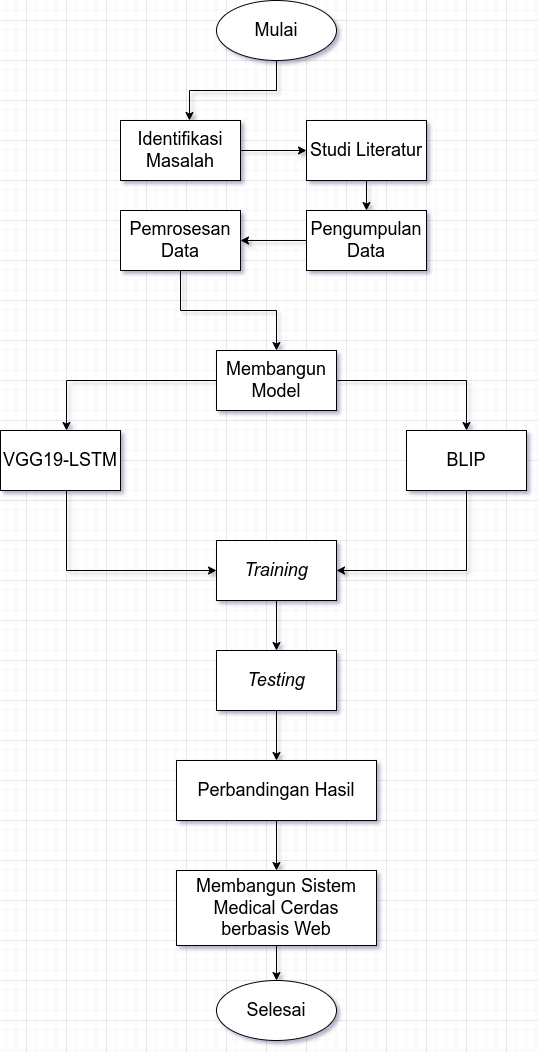
\includegraphics [width = 9cm, height= 16cm]{image/bab3/diagram_alir_penelitian8}}
\caption{Diagram alir penelitian}
\label{alur_penelitian}
\end{figure}

\subsection{Identifikasi Masalah}

\par Identifikasi masalah adalah proses awal dalam mengidentifikasi masalah yang akan diselesaikan dalam penelitian ini. Identifikasi masalah meliputi latar belakang masalah, rumusan masalah, tujuan penelitian serta manfaat yang dapat dihasilkan dari penelitian ini.

\subsection{Studi Literatur}

\par Studi literatur dilakukan untuk memperoleh informasi mengenai penelitian yang sudah dilakukan sebelumnya. Dalam tahapan ini terdiri dari banyak kegiatan yaitu membaca referensi yang berkaitan dengan penelitian ini, membaca jurnal atau buku untuk menambah wawasan, sehingga dapat memperoleh informasi yang dibutuhkan untuk penelitian ini.



\subsection{Pengumpulan Data}

\par Penelitian tugas akhir ini menggunakan data dari \textit{\textit{dataset}} PathVQA dan VQA-RAD. Pengumpulan \textit{\textit{dataset}} dilakukan dengan mengunduh data dari platform Hugging Face. Sampel kedua data ini bisa dilihat pada Gambar \ref{data_pathvqa} dan Gambar \ref{data_vqa-rad}.

\begin{figure}[H]
    \centering
    {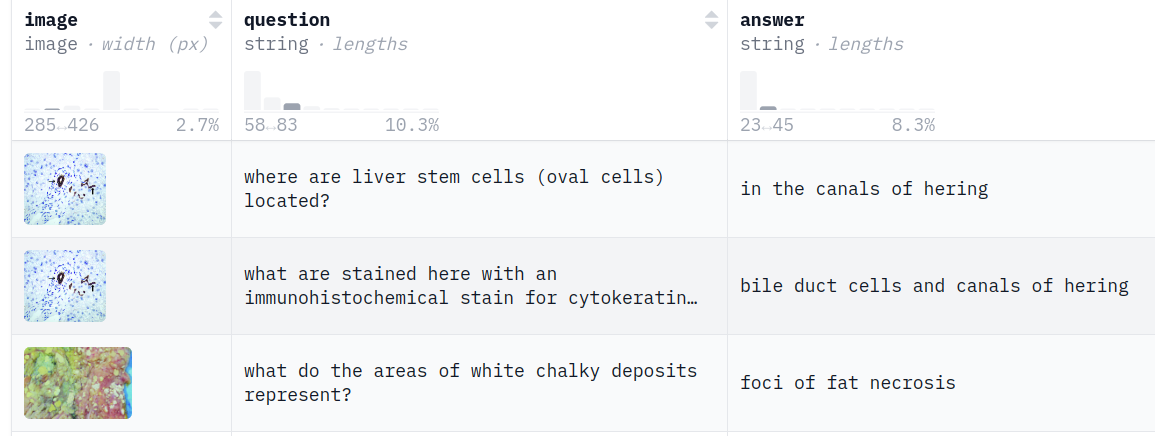
\includegraphics[width=\textwidth, height = 7cm]{image/bab3/pathvqa-sample.png}}
    \caption{Sampel data PathVQA}
    \label{data_pathvqa}
\end{figure}


\begin{figure}[H]
    \centering
    {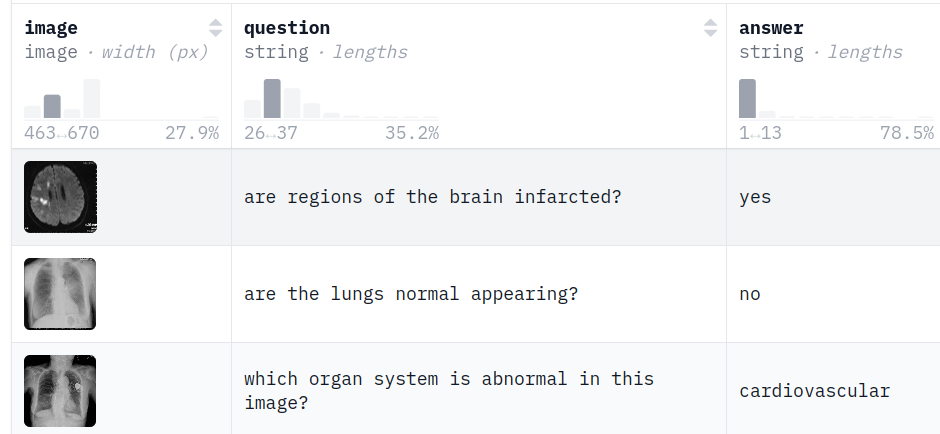
\includegraphics[width=\textwidth, height = 7cm]{image/bab3/vqarad-sample.png}}
    \caption{Sampel data VQA-RAD}
    \label{data_vqa-rad}
\end{figure}


\subsection{Pemrosesan Data}

\par Pada bagian ini, dilakukan pemrosesan data dengan tujuan menyelaraskan dan menyusun \textit{dataset} yang diperlukan untuk model \textit{Visual Question Answering} (VQA). Proses ini melibatkan penggabungan antara data visual, seperti gambar, dan data teks, berupa pertanyaan yang berkaitan. Pemrosesan data bertujuan untuk mengkonversi informasi kompleks dari kedua modalitas ini ke dalam format yang dapat dicerna oleh model. Dengan melakukan pemrosesan data ini, kita menciptakan representasi yang optimal untuk menyajikan informasi visual dan teks kepada model VQA. Hasilnya adalah \textit{dataset} yang kohesif dan siap digunakan untuk melatih model VQA agar mampu memberikan jawaban yang tepat terhadap pertanyaan yang diajukan berdasarkan konteks visual yang diberikan. Adapun pemrosesan data yang dilakukan mencakup pemrosesan gambar dan teks.


\begin{enumerate}

\item{\textit{Case Folding}}

\par Pada bagian ini proses \textit{case folding} dilakukan untuk mengubah semua karakter dalam teks menjadi huruf kecil. Hal ini dilakukan untuk menghindari duplikasi kata yang sama dengan huruf besar dan kecil. Tabel \ref{tab:case-folding} menunjukkan contoh proses \textit{case folding}.

\begin{table}[H]
    \centering
    \caption{Proses \textit{case folding}}
    \label{tab:case-folding}
    \begin{tabular}{|l|l|}
    \hline
    \multicolumn{1}{|c|}{\textbf{Sebelum}} & \multicolumn{1}{c|}{\textbf{Sesudah}} \\ \hline
    The Quick Brown Fox JUMPS              & the quick brown fox jumps             \\ \hline
    \end{tabular}
\end{table}


\item{\textit{Remove Punctuation}}

\par Pada bagian ini proses \textit{remove punctuation} dilakukan untuk menghapus tanda baca dalam teks. Hal ini dilakukan untuk mengurangi kompleksitas kata dalam teks. Tabel \ref{tab:remove-punctuation} menunjukkan contoh proses \textit{remove punctuation}.

\begin{table}[H]
    \centering
    \caption{Proses \textit{remove punctuation}}
    \label{tab:remove-punctuation}
    \begin{tabular}{|l|l|}
    \hline
    \multicolumn{1}{|c|}{\textbf{Sebelum}} & \multicolumn{1}{c|}{\textbf{Sesudah}} \\ \hline
    She said, 'Hello!' and waved           & She said Hello and waved              \\ \hline
    \end{tabular}
\end{table}

\item{\textit{Stemming}}

\par Pada bagian ini proses \textit{stemming} dilakukan untuk mengubah kata-kata dalam teks menjadi kata dasar. Hal ini dilakukan untuk mengurangi kompleksitas kata dalam teks. Tabel \ref{tab:stemming-text} menunjukkan contoh proses \textit{stemming-text}.

\begin{table}[H]
    \centering
    \caption{Proses \textit{stemming}}
    \label{tab:stemming-text}
    \begin{tabular}{|l|l|}
    \hline
    \multicolumn{1}{|c|}{\textbf{Sebelum}} & \multicolumn{1}{c|}{\textbf{Sesudah}} \\ \hline
    running quickly in the park            & run quick in the park                 \\ \hline
    \end{tabular}
\end{table}

\item{Tokenisasi}

\par Pada bagian ini proses tokenisasi dilakukan untuk memecah teks menjadi token-token yang lebih kecil. Hal ini dilakukan untuk mempermudah model VQA memahami dan memproses secara efektif. Tabel \ref{tab:tokenisasi} menunjukkan contoh proses tokenisasi.

\begin{table}[H]
    \centering
    \caption{Proses tokenisasi}
    \label{tab:tokenisasi}
    \begin{tabular}{|l|l|}
    \hline
    \multicolumn{1}{|c|}{\textbf{Sebelum}} & \multicolumn{1}{c|}{\textbf{Sesudah}}  \\ \hline
    The cat in the hat                     & {[}The, cat, in, the, hat{]} \\ \hline
    \end{tabular}
\end{table}

\item{Pemrosesan Gambar}

\par Pada bagian ini proses pemrosesan gambar dilakukan menyamaratakan format gambar. Hal ini dilakukan untuk mempermudah proses pemrosesan data dan mempersiapkan data agar siap digunakan untuk melatih model VQA.


\end{enumerate}

\subsection{Membangun Model}

\par Proses membangun model VQA ini menggunakan arsitektur VGG19-LSTM dan BLIP. Pada VGG19-LSTM, terdapat dua tahap pemrosesan, yaitu ekstraksi fitur gambar menggunakan VGG19 dan pemrosesan teks menggunakan LSTM. Sedangkan pada BLIP, terdapat dua \textit{encoder}, yaitu \textit{image encoder} dan \textit{text encoder}, yang digunakan untuk mengolah data gambar dan teks. Dalam BLIP, \textit{image encoder} menggunakan \textit{Vision Transformer} (ViT), sedangkan \textit{text encoder} menggunakan \textit{transformer encoder}. Proses ini bertujuan untuk membangun model VQA yang mampu memberikan jawaban yang tepat terhadap pertanyaan yang diberikan berdasarkan konteks visual yang diberikan.



\subsection{Melatih Model}

\par Tahapan pada pelatihan model ini menggunakan arsitektur VGG19-LSTM dan BLIP. Pada tahap ini akan dilakukan suatu metode yang bertujuan untuk mengubah nilai atau parameter yang ada pada suatu arsitektur, Proses ini disebut sebagai \textit{hyperparameter tuning}. \textit{Hyperparameter} ini mengacu pada parameter yang tidak dapat diubah ketika proses pelatihan model berjalan, contohnya seperti jumlah \textit{hidden layer}, nilai \textit{epoch}, \textit{batch size}, \textit{learning rate} pada fungsi optimasi, dan lain-lain. \textit{Hyperparameter tuning} ini dilakukan untuk mencari kombinasi nilai yang optimal untuk parameter-parameter tersebut \citep{yu2020hyper}.

\subsection{Perbandingan Hasil}

\par Setelah proses pelatihan model selesai, maka dilakukan perbandingan hasil dari kedua model yang telah dibangun dengan menggunakan metrik evaluasi yaitu akurasi dan \textit{Bilingual Evaluation Understudy} (BLEU). Pada metrik BLEU, penulis akan menggunakan BLEU-1, BLEU-2, dan BLEU-3, bilangan pada nama BLEU menunjukkan jumlah n-gram yang digunakan. Kedua metrik ini digunakan untuk mengevaluasi kinerja dari model VQA yang telah dilatih. Perbandingan hasil ini dilakukan dengan cara menguji kedua model menggunakan data uji yang telah disiapkan. Hasil dari perbandingan ini akan digunakan untuk menentukan model mana yang lebih baik dalam memberikan jawaban dari pertanyaan yang diberikan. 




\subsection{Membangun Sistem Medis Cerdas Berbasis Web}

\par Model yang telah siap dilatih akan di \textit{deploy} ke dalam sistem medis cerdas berbasis web. Dalam proses membangun \textit{website} ini meliputi pengembangan halaman tampilan yang bisa menerima dua \textit{input} yaitu gambar dan pertanyaan dari pengguna. Setelah itu mengembangkan bagian \textit{backend} untuk mengolah kedua \textit{input} tersebut dan memasukkannya ke dalam model yang telah dibangun sebelumnya. Setelah model menghasilkan jawaban, maka jawaban tersebut akan dikirimkan kembali ke halaman tampilan untuk ditampilkan kepada pengguna.




%-----------------------------------------------------------------------------%

% Baris ini digunakan untuk membantu dalam melakukan sitasi
% Karena diapit dengan comment, maka baris ini akan diabaikan
% oleh compiler LaTeX.
\begin{comment}
\bibliography{daftar-pustaka}
\end{comment}
